\section{Sensors} \label{cha:sensorChapter}
%Explain the need for sensors
To acquire relevant data from the golf course, and to enable processing of this data in a digital domain, a sensor is needed.
The sensors must be capable of measuring data, and returning a value, either as a digital or analog signal that can be processed by a computation unit.
As multiple sensors are needed, the price point is considered relevant, as it will cause the overall cost of the solution to grow.

There exist several kind of sensors, such as soil pH sensor, soil density sensor, temperature sensor and many more. In this project only the soil moisture sensor will be covered, since adding a different sensor would be trivial.

\subsection{Moisture Sensor}
To obtain information about the moisture of soil on the golf course, a moisture sensor is needed.
The moisture can change relatively quickly depending on rain and and type of soil.
The moisture sensor used in this project is a Arduino Soil Hygrometer Detection Module Soil Moisture Sensor.
The sensor operates with a voltage of 3.3V to 5V.
It has dual output, both digital and analog, with analog being the most accurate.
The digital output is in the form low(0) and high(1), while the analog output range from low(0V) to high(5V) \cite{moisture}.

When the output is high, the moisture content of the soil is high, while a low output means a low moisture content.
Calibration is needed when there are several sensors which should provide the same range of moisture.
Figure \ref{fig:moisture_figure} shows the moisture sensor, with the fork being the actual sensor, and the circuit board being the converter and calibrator. 

\begin{figure}[H]
\centering
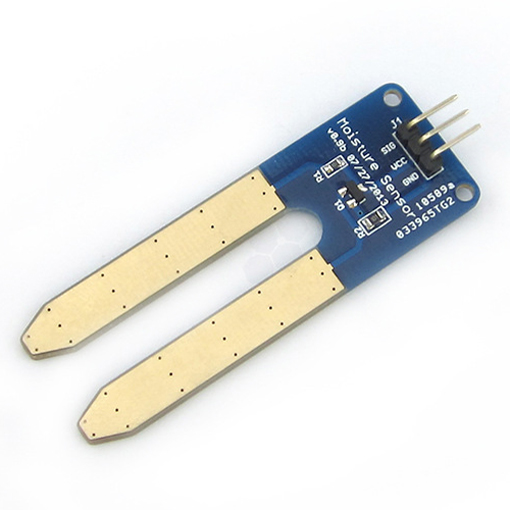
\includegraphics[width=0.6\textwidth]{chapters/analysis/figs/soilMoistureSensor.jpg}
\caption{Soil moisture sensor.}
\label{fig:moisture_figure}
\end{figure}
